%%%%%%%%%%%%%%%%%%%%%%%%%%%%%%%%%%%%%%%%%%%%%%%%%%%%%%%%%%%%%%%%%%%%%%%%%%%%%%%%%%%%%%%%%%%%%%%%%%%%%%%%%%
%Write by:ShuwenHe
%Date:20230613
%%%%%%%%%%%%%%%%%%%%%%%%%%%%%%%%%%%%%%%%%%%%%%%%%%%%%%%%%%%%%%%%%%%%%%%%%%%%%%%%%%%%%%%%%%%%%%%%%%%%%%%%%%

%%%%%%%%%%%%%%%%%%%%%%%%%%%%%%%%%%%%%%%%%%%%%%%%%%%%%%%%%%%%%%%%%%%%%%%%%%%%%%%%%%%%%%%%%%%%%%%%%%%%%%%%%%
\documentclass[12pt,twiside,a4paper]{ctexbook}
\usepackage[centertags]{amsmath}
\usepackage{amsfonts}
\usepackage{amsthm}
\usepackage{newlfont}
\usepackage{makeidx}
\usepackage{wasysym}
\usepackage{geometry} 
\usepackage{graphics}
\usepackage{slashbox} 
\usepackage{fancyhdr} 
\usepackage[pdftex]{graphicx}
\usepackage{epstopdf}
\usepackage{cite}
\usepackage{listings}
\usepackage{tocbibind}
\usepackage[numbers,sort&compress]{natbib}

\setlength\parskip{\baselineskip}
\setcounter{tocdepth}{8} % 生成目录层级
\setcounter{secnumdepth}{4}
\renewcommand\thesection{\arabic{section}}
\usepackage[pdfstartview=FitH,CJKbookmarks=true,bookmarks,bookmarksnumbered=true,
    colorlinks=true,citecolor=black,linkcolor=black,anchorcolor=green,urlcolor=black]{hyperref}
\usepackage{titlesec}
\usepackage{tabularx}
\titleformat{\chapter}[display]{\normalfont\huge\bfseries\center}{\chaptertitlename}{1pt}{\Huge}
\titleformat{\section}{\normalfont\Large\bfseries}{\thesection}{1em}{}
\titleformat{\subsection}{\normalfont\large\bfseries}{\thesubsection}{1em}{}
\titleformat{\subsubsection}{\normalfont\normalsize\bfseries}{\thesubsubsection}{1em}{}
\titleformat{\paragraph}[runin]{\normalfont\normalsize\bfseries}{\theparagraph}{1em}{}
\titleformat{\subparagraph}[runin]{\normalfont\normalsize\bfseries}{\thesubparagraph}{1em}{}
\titlespacing*{\chapter} {0pt}{10pt}{10pt}
\titlespacing*{\section} {0pt}{0.5ex plus 1ex minus .2ex}{0.3ex plus .2ex}
\titlespacing*{\subsection} {0pt}{0.25ex plus 1ex minus .1ex}{0.5ex plus .1ex}
\titlespacing*{\subsubsection}{0pt}{3.25ex plus 1ex minus .2ex}{1.5ex plus .2ex}
\titlespacing*{\paragraph} {0pt}{3.25ex plus 1ex minus .2ex}{1em}
\titlespacing*{\subparagraph} {\parindent}{3.25ex plus 1ex minus .2ex}{1em}
\numberwithin{chapter}{part}
\geometry{left=2.0cm,right=20mm,top=25mm,bottom=25mm}
\let\cleardoublepage\clearpage
%%%%%%%%%%%%%%%%%%%%%%%%%%%%%%%%%%%%%%%%%%%%%%%%%%%%%%%%%%%%%%%%%%%%%%%%%%%%%%%%%%%%%%%%%%%%%%%%%%%%%%%%%%

%%%%%%%%%%%%%%%%%%%%%%%%%%%%%%%%%%%%%%%%%%%%%%%%%%%%%%%%%%%%%%%%%%%%%%%%%%%%%%%%%%%%%%%%%%%%%%%%%%%%%%%%%%
%mathematics
\usepackage{amssymb}
\usepackage{diagbox}
%%%%%%%%%%%%%%%%%%%%%%%%%%%%%%%%%%%%%%%%%%%%%%%%%%%%%%%%%%%%%%%%%%%%%%%%%%%%%%%%%%%%%%%%%%%%%%%%%%%%%%%%%%

%%%%%%%%%%%%%%%%%%%%%%%%%%%%%%%%%%%%%%%%%%%%%%%%%%%%%%%%%%%%%%%%%%%%%%%%%%%%%%%%%%%%%%%%%%%%%%%%%%%%%%%%%%
%
%%%%%%%%%%%%%%%%%%%%%%%%%%%%%%%%%%%%%%%%%%%%%%%%%%%%%%%%%%%%%%%%%%%%%%%%%%%%%%%%%%%%%%%%%%%%%%%%%%%%%%%%%%

%%%%%%%%%%%%%%%%%%%%%%%%%%%%%%%%%%%%%%%%%%%%%%%%%%%%%%%%%%%%%%%%%%%%%%%%%%%%%%%%%%%%%%%%%%%%%%%%%%%%%%%%%%
%
\usepackage{tipa} % 音标
%%%%%%%%%%%%%%%%%%%%%%%%%%%%%%%%%%%%%%%%%%%%%%%%%%%%%%%%%%%%%%%%%%%%%%%%%%%%%%%%%%%%%%%%%%%%%%%%%%%%%%%%%%

%%%%%%%%%%%%%%%%%%%%%%%%%%%%%%%%%%%%%%%%%%%%%%%%%%%%%%%%%%%%%%%%%%%%%%%%%%%%%%%%%%%%%%%%%%%%%%%%%%%%%%%%%%
\begin{document}
%%%%%%%%%%%%%%%%%%%%%%%%%%%%%%%%%%%%%%%%%%%%%%%%%%%%%%%%%%%%%%%%%%%%%%%%%%%%%%%%%%%%%%%%%%%%%%%%%%%%%%%%%%

\author
{
ShuwenHe\\
何书文\\
1201220707@pku.edu.cn
}

%%%%%%%%%%%%%%%%%%%%%%%%%%%%%%%%%%%%%%%%%%%%%%%%%%%%%%%%%%%%%%%%%%%%%%%%%%%%%%%%%%%%%%%%%%%%%%%%%%%%%%%%%%
%\centerline{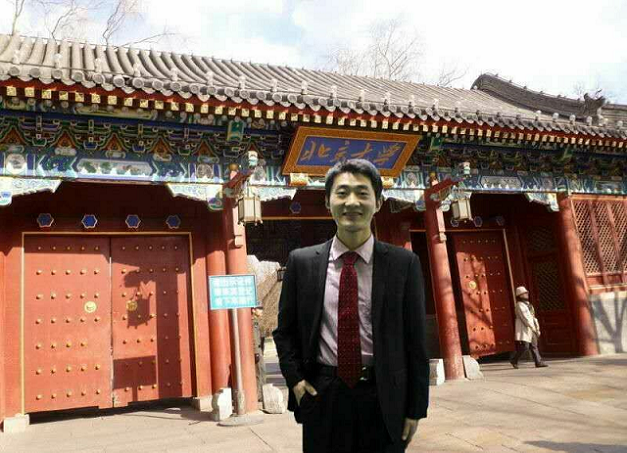
\includegraphics{shuwenhe.png}}
%写好一本书:工匠精神!用心打造!夜深写于北京大学图书馆。作者亲自一线带课,所带学生多人保送或考入清华北大,根据多年清华附中、101中学、人大附中、北大附中、十一学校,考试真题分析经验所得。用此书考上心目中名校学生无数!何书文北京大学硕士,资深数学名师、信息学竞赛算法名师,所带学生多名考入人大附中早培、清华附中优才、101 实验班、北大附中实验班等名校。全国中学数学联赛、全国中学数学竞赛的辅导老师,全国NOI、CSP信息学竞赛辅导名师。何书文老师在北京大学学习期间立志从事教育事业,帮学生授业解惑。何书文老师小学期间学习奥数,并多次获奖,为以后的学习与研究打下良好基础。何书文 老师在中学阶段数学、物理均获奖。何书文老师在小学中学期间一直为数学课代表,中小学大学期间担任班长,何书文老师在北京大学被选为科技一苑苑长,组织北大同学积极参与校各项活动,积极参与校学生会工作,何书文老师被北京大学评为优秀入党积极分子.何书文老师经常参加北京大学数学课题的研讨班。何书文 老师是北京大学数学系暑期学校全国选出40 名优秀中青年数学人才之一,参加伦敦国王学院、美国杜克大学、美国纽约大学、加拿大多伦多大学教授组成的学术研讨班,研究PDE(偏微分方程),量子力学方面的数学课题的研究工作,并获得优异成绩结业。何书文老师作为项目经理用数学建模方法给大型企业开发软件,用数学方法规划提高企业产能协作效率。何书文 老师致力于数学方面的教学与研究工作,所带多名孩子已经被点优才进入清华附中创新班,101 实验班,人大附中早培班,是家长值得信赖的老师。考上学生继续跟随何书文老师学习全国数学联赛,全国数学竞赛系列课程,同时学习NOI、IOI、ACM算法编程竞赛。
%%%%%%%%%%%%%%%%%%%%%%%%%%%%%%%%%%%%%%%%%%%%%%%%%%%%%%%%%%%%%%%%%%%%%%%%%%%%%%%%%%%%%%%%%%%%%%%%%%%%%%%%%%

%%%%%%%%%%%%%%%%%%%%%%%%%%%%%%%%%%%%%%%%%%%%%%%%%%%%%%%%%%%%%%%%%%%%%%%%%%%%%%%%%%%%%%%%%%%%%%%%%%%%%%%%%%
\title{English}
\maketitle
\tableofcontents % 显示目录
\newpage
\pagestyle{fancy}
%%%%%%%%%%%%%%%%%%%%%%%%%%%%%%%%%%%%%%%%%%%%%%%%%%%%%%%%%%%%%%%%%%%%%%%%%%%%%%%%%%%%%%%%%%%%%%%%%%%%%%%%%%

%\lhead{
\includegraphics{shuwenedu.png}}
%\rhead{科技特长生升学规划 何校长 电话微信15010729356}
%\lfoot{
\includegraphics{pku.png}算法第一人北大何书文}
%\rfoot{改变您家孩子命运的老师}
%%%%%%%%%%%%%%%%%%%%%%%%%%%%%%%%%%%%%%%%%%%%%%%%%%%%%%%%%%%%%%%%%%%%%%%%%%%%%%%%%%%%%%%%%%%%%%%%%%%%%%%%%%

%%%%%%%%%%%%%%%%%%%%%%%%%%%%%%%%%%%%%%%%%%%%%%%%%%%%%%%%%%%%%%%%%%%%%%%%%%%%%%%%%%%%%%%%%%%%%%%%%%%%%%%%%%
\begin{center}
\begin{tabularx}{\textwidth}{|c|X|}
\hline
\textbf{英语音标} & \textbf{TeX音标} \\
\hline
\textipa{I} & \verb|\textipa{I}| \\
e & \verb|\textipa{e}| \\
\textipa{\textepsilon} & \verb|\textipa{\textepsilon}| \\
\textipa{A}& \verb|\textipa{A}| \\
\textipa{o} & \verb|\textipa{o}| \\
\textipa{U} & \verb|\textipa{U}| \\
u & \verb|\textipa{u}| \\
ə & \verb|\textipa{@}| \\
\textipa{g} & \verb|\textipa{g}| \\
\textipa{T} & \verb|\textipa{T}| \\
ð & \verb|\textipa{D}| \\
\textipa{S} & \verb|\textipa{S}| \\
\textipa{Z} & \verb|\textipa{Z}| \\
ŋ & \verb|\textipa{N}| \\
\textturnscripta & \verb|\textipa{\textturnscripta}|\\
\textipa{\textopeno} & \verb|\textipa{\textopeno}|\\
\textprimstress & \verb|\textprimstress|\\
\textipa{\textsecstress} & \verb|\textipa{\textsecstress}|\\
\textipa{\textlengthmark} & \verb|\textlengthmark|\\
\hline
\end{tabularx}
\end{center}

\section{ai}
\begin{tabular}{|c|c|c|c|c|}
\hline
英文 & 音标 & 中文 & 词根词缀 & 词组\\
\hline
artificial&/ˌɑːrtɪˈfɪʃ(ə)l/&adj.人工的&&artificial intelligence人工智能\\
intelligence&&智力&词根词缀: intel- 之间 , 中间 + -lig- 诵读 + -ence 名词词尾&\\
absolutely && adv.绝对& & \\
adjacency & /ə\textprimstress d\textipa{Z}e\textipa{I}sənsi/ & n. 邻接 & & adjacency list 邻接表 adjacency matrix 邻接矩阵 \\
assign & /əˈsaɪn/ & v. 分配 & & \\
algorithm & /\textprimstress æl\textipa{g}ər\textipa{I}ðəm/ & n. 算法 & & \\
\hline
\end{tabular}

\section{space}
\begin{tabular}{|c|c|c|c|}
\hline
英文 & 音标 & 中文 & 词根\\
\hline
silicon valley&&硅谷&\\
system& &系统& \\
\hline
\end{tabular}

\section{system}
\begin{tabular}{|c|c|c|c|c|}
\hline
英文 & 音标 & 中文 & 词根词缀 & 词组\\
\hline
community&/kəˈmjuːnəti/&n.社区&com共同+mun公共+ity名词词尾&\\ 
architecture&/ˈɑːkɪtektʃə(r)/&n.架构&-arch- 统治 + -i- + tect ( -techn- )技术 + -ure 名词词尾&\\
bipartite & /ba\textipa{I}\textprimstress p\textipa{A}\textlengthmark ta\textipa{I}t/ & adj. 二分的 & & bipartite graph 二分图\\
barn & /bɑːn/ & n. 谷仓 & & born出生\\
\hline
\end{tabular}

\section{money}
\begin{tabular}{|c|c|c|c|c|}
\hline
英文 & 音标 & 中文 & 词根词缀 & 词组\\
\hline
billion&/ˈbɪljən/&n.十亿&前缀 bi-, 二。 million, 百万。字面意思是万亿,现通常指十亿
词根词缀: bi- 两 , 二 + million → billion&\\
column & /ˈkɒləm/ & n. 列 & &\\
contest & /ˈkɒntest/ & n. 比赛 & &\\
competition& /ˌkɒmpəˈtɪʃ(ə)n/ & n. 竞赛 & &\\
candy & /\textprimstress kændi/ & n. 糖果 & &\\
constant & /ˈkɒnstənt/ & n. 常数 & & constant value 常数值\\
complement & /ˈkɒmplɪment/ & n. 补集 & &\\
\hline
\end{tabular}

\section{country}
\begin{tabular}{|c|c|c|c|c|}
\hline
英文 & 音标 & 中文 & 词根词缀 & 词组\\
\hline
france&/frɑːns/&n.法国& & \\
french&/frentʃ/&n.法国人法语& & \\
europe&/ˈjʊrəp/&n.欧洲& & \\
government&&n.政府&&\\
division&/dɪˈvɪʒ(ə)n/&n.除法&&\\
dijkstra & /ˈdaɪkstrə/ & n. 迪杰斯特拉 & & \\
directive & /dəˈrektɪv/ & n. 指令 & & preprocessor directive预处理器指令\\
declared & & & &\\
dynamic & /daɪˈnæmɪk/ & & &  dynamic prgramming动态规划\\
\hline
\end{tabular}

\section{person}
\begin{tabular}{|c|c|c|c|c|}
\hline
英文&音标&中文&词根&词组\\
\hline
engineer&/ˌendʒɪˈnɪə(r)/&工程师&gen生殖engine引擎er人&\\
energy&&能量&sustainable energy可持续能源&\\
engineer&&工程师&volunteer志愿者pioneer开拓者&\\
element & /\textprimstress el\textipa{I}mənt/ & n. 元素& &\\
logical expression &&&&\\
\hline
\end{tabular}

\section{electric car}
\begin{tabular}{|c|c|c|c|c|}
\hline
英文 & 音标 & 中文 & 词根词缀 & 词组\\
\hline
electric&/ɪˈlektrɪk/&电动的&&\\
electricity&/ɪˌlekˈtrɪsəti/&电力&&\\
focus on&&专注于&&\\
\hline
factorial & /fækˈtɔːriəl/ & n. [数] 阶乘 & &\\
\hline
\end{tabular}

\section{g}
\begin{tabular}{|c|c|c|c|}
\hline
词汇 & 音标 & 译意 & 词根词缀\\
\hline
generation& /ˌdʒenəˈreɪʃn/&一代&\\
greedy & /\textprimstress\textipa{g}ri\textlengthmark di/ & adj. 贪心的& \\
graph & /ɡrɑːf/ & adj. 贪心的& \\
\hline
\end{tabular}

\section{h}

\section{i}
\begin{tabular}{|c|c|c|c|c|}
\hline
英文 & 音标 & 中文 & 词根词缀 & 词组\\
internet&&n.互联网&&\\
innovation&/ˌɪnəˈveɪʃn/&n.创新&&\\
issue  & /ˈɪʃuː/ & n.问题&&big issue大问题\\
infinity  & /ɪnˈfɪnəti/ & n. 无穷 & &\\
increment & /\textprimstress\textipa{I}ŋkrəmənt/ & 自增 & in- 入 , 向内 + -cre- 生长 + -ment 名词词尾 &\\
implementation & /\textipa{\textsecstress}\textipa{I}mpl\textipa{I}men\textipa{\textprimstress}te\textipa{I}\textipa{S}(ə)n/ & n. 实现& &\\
International & & & International Phonetic Alphabet国际音标&\\
\hline
\end{tabular}

\section{j}
\section{k}
\section{l}
\begin{tabular}{|c|c|c|c|c|}
\hline
英文 & 音标 & 中文 & 词根词缀 & 词组\\
\hline
deep learning&&深度学习&&\\
machine learning&&机器学习&&\\
\hline
\end{tabular}
logical expression

\section{m}
\begin{tabular}{|c|c|c|c|c|}
\hline
英文 & 音标 & 中文 & 词根词缀 & 词组\\
\hline
mathematics & /\textipa{\textsecstress}mæ\textipa{T}ə\textprimstress mæt\textipa{I}ks/ & n. 算法 & &\\
modify & /\textprimstress m\textturnscripta d\textipa{I}fa\textipa{I}/ & v. 修改 &&\\
macro & /ˈmækrəʊ/ & n. (计算机)宏 & &  defines a macro定义一个宏\\
memorization & /ˌmeməˈrɪzeɪʃən/ & n. (计算机)宏 & &  memorization search 记忆搜索\\
\hline
\end{tabular}

\section{n}
\begin{tabular}{|c|c|c|c|c|}
\hline
英文 & 音标 & 中文 & 词根词缀 & 词组\\
\hline
nuked & /nju\textlengthmark kt/ & 核武器 & & bool nuked[maxN];\\
\hline
\end{tabular}

\section{o}
\begin{tabular}{|c|c|c|c|}
\hline
词汇 & 音标 & 译意 & 词根词缀\\
\hline
origin & /\textprimstress\textipa{\textopeno}\textipa{\textlengthmark}r\textipa{I}d\textipa{Z}\textipa{I}n/ & n. 起源& \\
original & /ə\textprimstress r\textipa{I}d\textipa{Z}ən(ə)l/ & adj. 起初的& \\
operator & /ˈɒpəreɪtə(r)/ & n.运算符 & \\
overload & /ˌəʊvəˈləʊd/ & v. 重载 & \\
operator & /ˈɒpəreɪtə(r)/ & n. 运算符 & \\
\hline
\end{tabular}

\section{p}
\begin{tabular}{|c|c|c|c|c|}
\hline
英文 & 音标 & 中文 & 词根词缀 & 词组\\
\hline
palindrome&/ˈpælɪndroʊm/&回文&palin重再drome跑&\\
priority & /praɪˈɔːrəti/ & v. 优先 &  & priority queue 优先队列\\
prune & /pru\textlengthmark n/ & v. 修剪 & &\\
prime & /praɪm/ & n. 素数 & &\\
proxy & /ˈprɒksi/ & n. 代理 & &\\
preprocessor & /ˌpriːˈprəʊsesə/ &预处理器&& preprocessor directive预处理器指令\\
positive & /ˈpɒzətɪv/ & n. 正数 & & positive value 正值\\
provide& /prəˈvaɪd/ & v. 提供 & & provided by 由......提供\\
permission&  & v. 提供 & & permission denied 权限拒绝\\
power& /ˈpaʊər/ & v. 提供 & & \\
pair& /peə(r)/ & v. 提供 & & \\
\hline
\end{tabular}

\section{q}
\section{r}
\begin{tabular}{|c|c|c|c|}
\hline
词汇 & 音标 & 译意 & 词根词缀\\
\hline
reference & /\textprimstress refrəns/ & 引用 & re- 回 + -fer- 拿取 + -ence 名词词尾\\
represent & /ˌreprɪˈzent/ & v.表示 &\\
recursive & /r\textipa{I}\textprimstress k\textipa{Z}\textipa{\textlengthmark}s\textipa{I}v/ & adj. [数] 递归的 &recur, 复发,再次发生,引申词义循环的\\
\hline
\end{tabular}

\section{t}
\begin{tabular}{|c|c|c|c|}
\hline
词汇 & 音标 & 译意 & 词根词缀\\
\hline
technology& &技术& \\
temp & /temp/ & 临时变量 & \\
\hline
\end{tabular}
\section{u}
\begin{tabular}{|c|c|c|c|c|}
\hline
英文 & 音标 & 中文 & 词根词缀 & 词组\\
\hline
unreachable & /ʌn'ri:tʃəbl/ & adj. 不能达到的 & &unreachable distance遥不可及的距离\\
\hline
\end{tabular}
\section{v}
\begin{tabular}{|c|c|c|c|c|}
\hline
词汇 & 音标 & 译意 & 词根词缀 & 复数\\
\hline
vector & /\textprimstress vektər/ & 向量 & &\\
vertex & /ˈvɜːteks/ & n. 顶点 & & vertices\\
valid & /ˈvælɪd/ & adj.合法的 & & \\
\hline
\end{tabular}
\section{w}
\section{x}
\section{y}
\section{z}

\clearpage
\end{document}
